\chapter{Diseño e Implementación del sistema basado en IoT}\label{cap: }

\addcontentsline{toc}{section}{Introducción}
        \textbf{\Large Introducción}\newline
        
    En este capítulo se comentan los pasos seguidos para la implementación del sistema: se realiza la descripción de este sistema, los sensores que incorpora y la descripción de los mismos. 
    Se explica la relación que se establece entre el IDE Arduino y los sensores, así como el empleo de la multiplexación. Además, se explican las características de la alimentación empleada y la evaluación económica del proyecto.
    
\section{Descripción del sistema} \label{descripcion_sistema}

    El sistema de supervisión se implementa sobre una prueba de concepto desarrollada para llevar a cabo la toma de la data de los sensores incorporados durante 4 meses para facilitar el continuar con la investigación e inferir los daños que las diferentes variables (temperatura, humedad, ruido y CO2) inciden en el deterioro de los objetos de la colección para los diferentes materiales que en ella se encuentran; esto según el análisis teórico desarrollado a lo largo del capítulo primero.

    Esta prueba de concepto (figura \ref{imag:prueba_concepto}) se dividió en 3 submódulos. En el submódulo 1 se encuentra el microcontrolador principal, en este caso un NodeMCU que tendrá interconectado a su vez un shield DS3231, un reloj de tiempo real para almacenar la fecha y hora de cada medición que se realice, así como un sensor SGP30 para la captura de los valores de CO2 dentro de la vitrina; estos datos son almacenados en una tarjeta SD por un shield de lector para este tipo de almacenamiento, además de contar con un sistema de respaldo interno de 2 baterías de litio para su funcionamiento continuo aunque existan fallos eléctricos, además de que las ubicaciones de las vitrinas se encuentre alejada de una toma de corriente eléctrica.

    Sin embargo, para casos extremos energéticos se agregó el submódulo 2 el cual es una batería de tipo power bank de 10A que va conectado también al submódulo 1 y puede ser recargado simultáneamente.

    Por su parte en el submódulo 3 se encuentran los 2 sensores para medir la temperatura, la humedad (DHT22) y el ruido a través de un sensor Grove de micrófono.\\
    
    \begin{figure}[H]
      \centering
      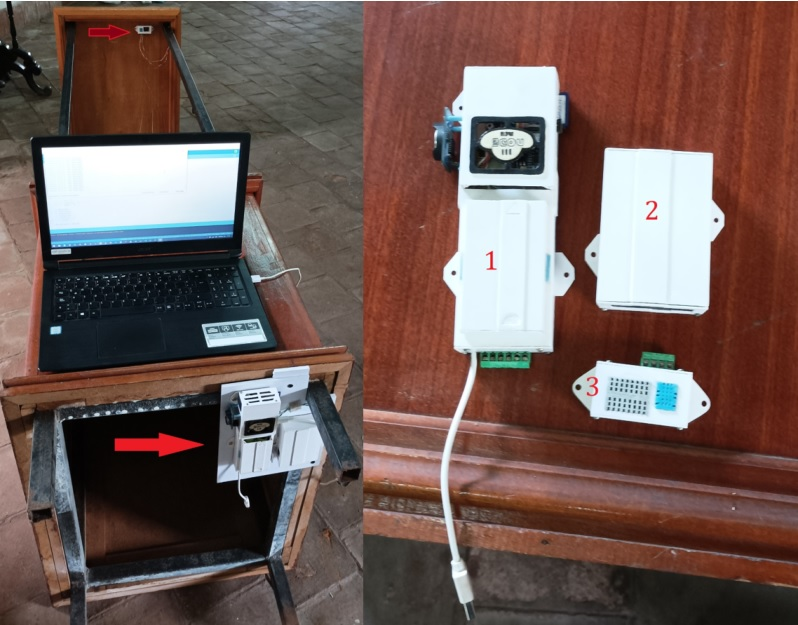
\includegraphics[width=7.5cm, height=6cm]{imagenes/prueba_concepto.jpg}
      \caption{Prueba de Concepto}
      \label{imag:prueba_concepto}
    \end{figure}

    Los submódulos fueron instalados en una sola vitrina y de manera separada a conveniencia de los investigadores y los especialistas del museo, el submodulo 1 y 2 se optó por ubicarlos en la parte baja de la vitrina (figura \ref{imag:ubicacion_submodulos1y2_vitrina}) en aras de que no rompiera el ambiente artístico de la colección,
    y el submódulo 3 es ubicado en la parte superior de la vitrina (figura \ref{imag:ubicacion_submodulo3}) para recolectar la mayor cantidad de información posible.

    \begin{figure}[H]
        \centering
        \begin{subfigure}[b]{0.45\linewidth}
        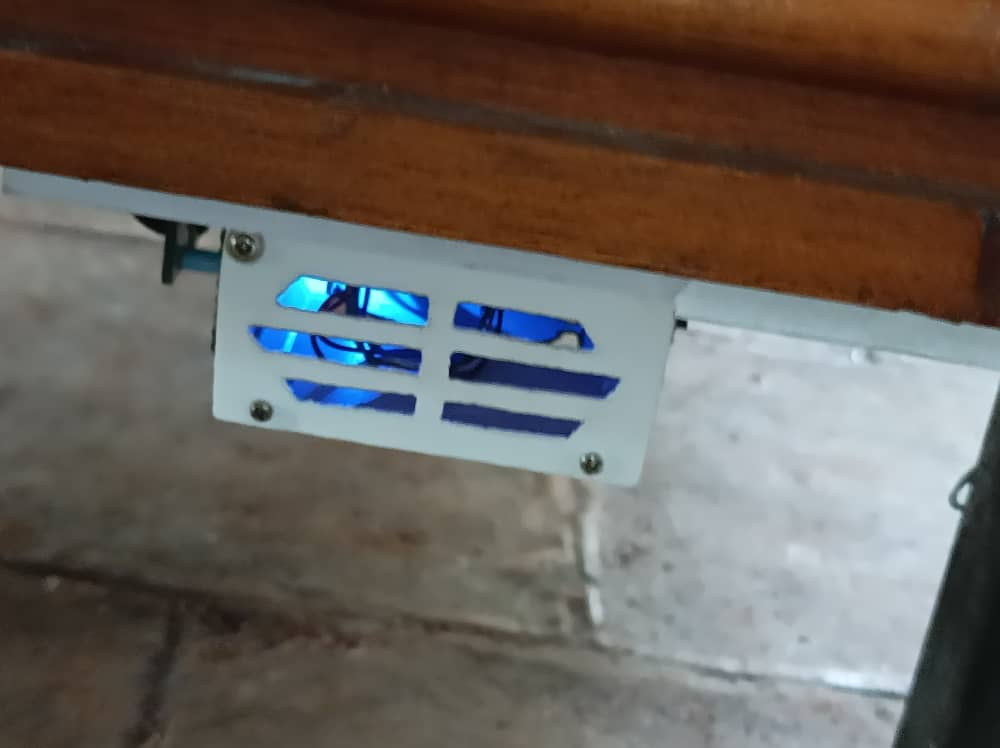
\includegraphics[width=\linewidth]{imagenes/submodulo 1.jpg}
        \caption{Ubicación submódulo 1}
        \label{imag:ubicacion_submodulo1}
    \end{subfigure}
    \begin{subfigure}[b]{0.45\linewidth}
        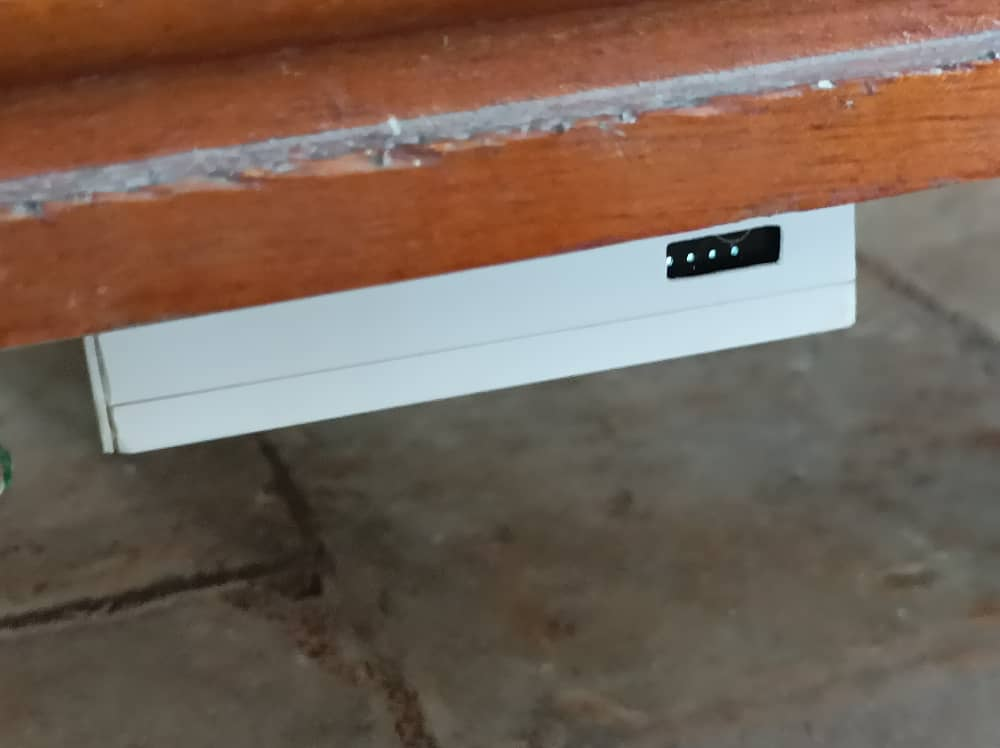
\includegraphics[width=\linewidth]{imagenes/submodulo 2.jpg}
        \caption{Ubicación submódulo 2}
        \label{imag:ubicacion_submodulo2}
    \end{subfigure}
        \caption{Ubicación de los submódulos 1 y 2 en la vitrina}
        \label{imag:ubicacion_submodulos1y2_vitrina}
    \end{figure}

    \begin{figure}[H]
        \centering
        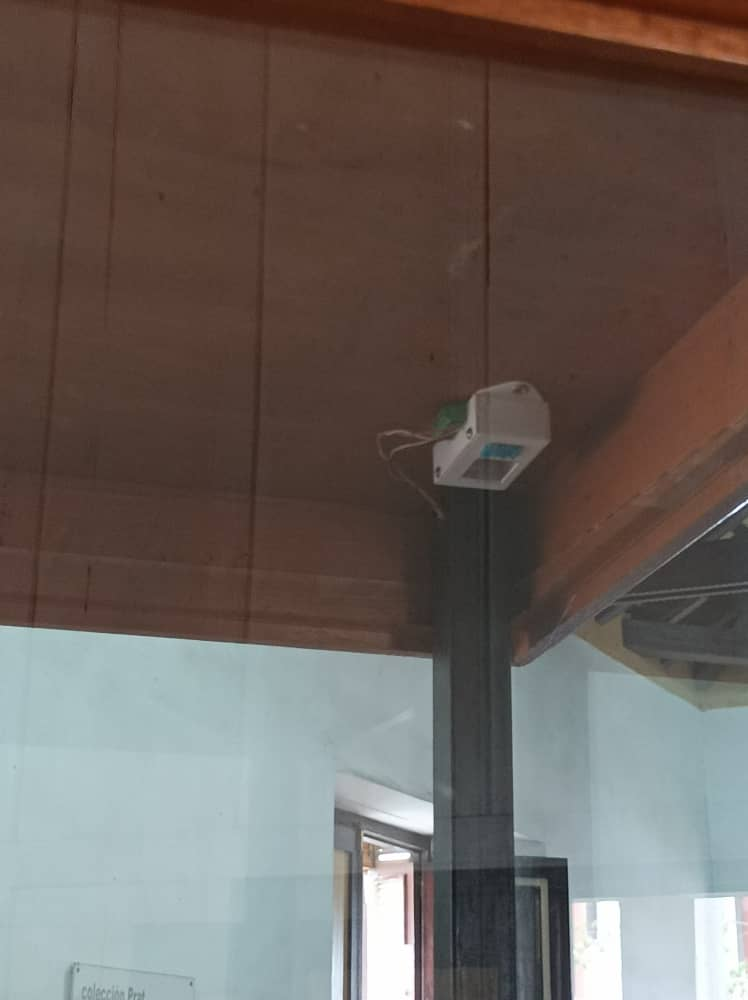
\includegraphics[width=7cm, height=6cm]{imagenes/submodulo 3.jpg}
        \caption{Ubicación submódulo 3}
        \label{imag:ubicacion_submodulo3}
    \end{figure}

    \subsection{Nuevo prototipo de Nodo} \label{subsec:nuevo_prototipo_nodo}

    La solución implementada a través de la prueba de concepto permitió obtener la data de cuatro sensores de los 9 previstos durante 4 meses lo que ha posibilitado continuar la investigación para inferir
    los daños que las diferentes variables (temperatura, humedad, ruido y CO2) inciden en el deterioro de los objetos de la colección para los diferentes materiales que en ella se encuentran.

    En base a esto se diseñó una placa de circuito impreso que estará presente en los Nodos (epígrafe \ref{subsec: nodos}) de las vitrinas.
    Este diseño posee características genéricas brinando la posibilidad de añadir o quitar sensores conforme a la ubicación del hardware.

    \newpage

    Este hardware corrige la deficiencias obtenidas durante la prueba de concepto, tales como:
      \begin{enumerate}
        \item Alto consumo de energía.
        \item Difícil acceso a los sensores y manipulación de los mismos.
        \item Limitación de entradas/salidas analógicas.
      \end{enumerate}

    En la figura \ref{imag:placa_impresa} se muestra el esquemático del diseño de la placa, y una representación gráfica brindada por el sofware de diseño de circuitos impresos KiCad.

    \begin{figure}[H]
        \centering
        \begin{subfigure}[b]{0.45\linewidth}
        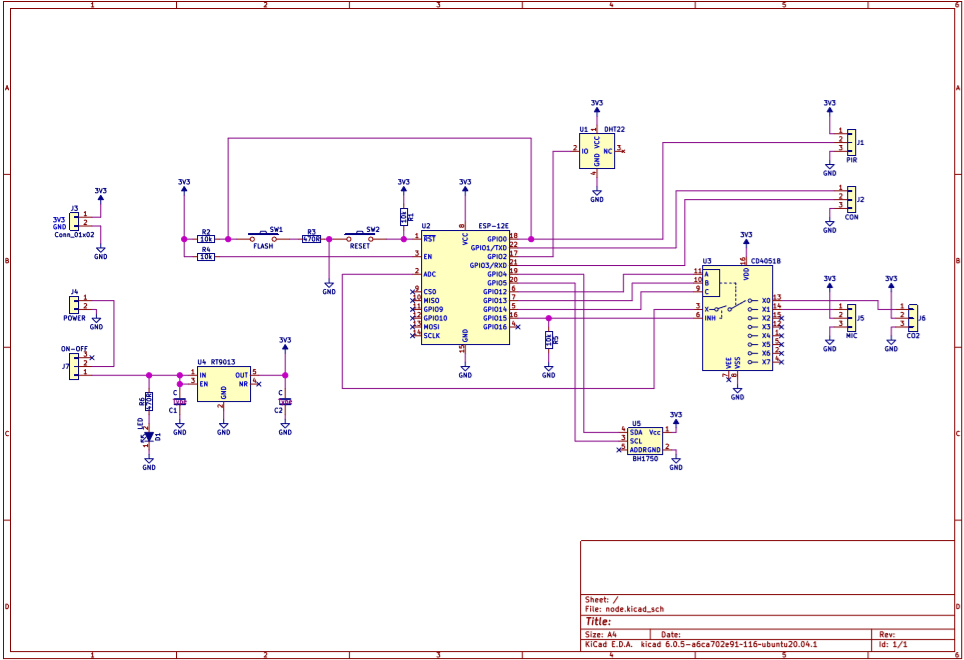
\includegraphics[width=\linewidth, height=5cm]{imagenes/esquematico nodo.jpg}
        \caption{Esquemático placa}
        \label{imag:esquematico_placa}
    \end{subfigure}
    \begin{subfigure}[b]{0.45\linewidth}
        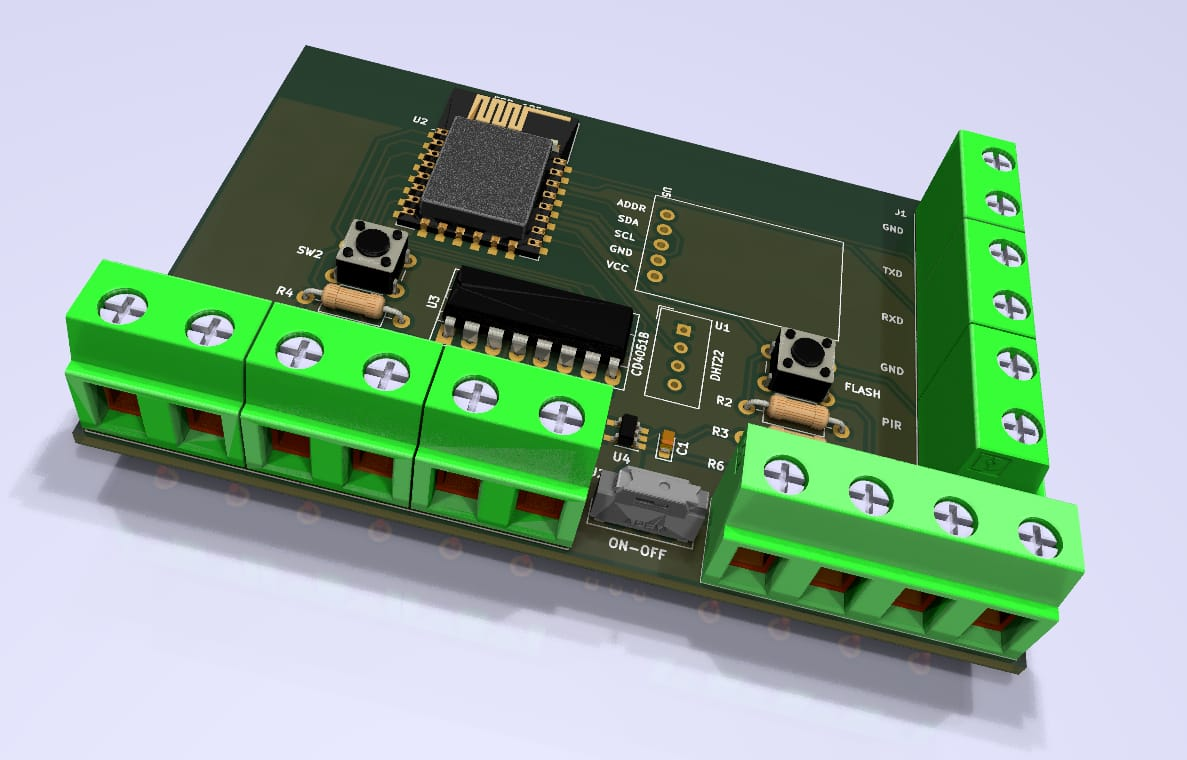
\includegraphics[width=\linewidth, height=5cm]{imagenes/vista 3D.jpg}
        \caption{Vista 3D placa}
        \label{imag:vista3D_placa}
    \end{subfigure}
        \caption{Placa para Nodos en las vitrinas (Ver anexo ...)}
        \label{imag:placa_impresa}
    \end{figure}


\section{Sensores} \label{sec:sensores}

    La secuencia de sensores pertenecientes al sistema es selecta, puesto que se tomaron los sensores teniendo en cuenta varios elementos:

    \begin{itemize}
        \item Variable a medir
        \item Rango de medición
        \item Precisión
        \item Voltaje de alimentación
        \item Corriente de alimentación
        \item Precio
    \end{itemize}

En la tabla \ref{tab:relacion_sensores} se relaciona el sensor a emplear según la variable a medir.

    \begin{table}[h]
        \centering
        \caption{Relación sensores}
        \label{tab:relacion_sensores}
        \begin{tabular}{|l|l|l|}
        \hline
        \cellcolor[HTML]{9698ED}                      & \cellcolor[HTML]{9698ED}                           & \cellcolor[HTML]{9698ED}                         \\
        \multirow{-2}{*}{\cellcolor[HTML]{9698ED}No.} & \multirow{-2}{*}{\cellcolor[HTML]{9698ED}Variable} & \multirow{-2}{*}{\cellcolor[HTML]{9698ED}Sensor} \\ \hline
        1                                             & Temperatura                                        & DHT22                                            \\ \hline
        2                                             & Humedad                                            & DHT22                                            \\ \hline
        3                                             & CO2                                                & SGP30                                            \\ \hline
        4                                             & Vibración                                          & TZT-LM393                                        \\ \hline
        5                                             & Calidad de Aire (polución)                         & ZP07-MP503                                       \\ \hline
        6                                             & Intensidad luminosa                                & BH1750                                           \\ \hline
        \end{tabular}
    \end{table}

Estos sensores estarán dispuestos en zonas específicas dentro de la colección, dígase en vitrinas o, para la captura de datos, en las salas.
Esto permite tener datos de dentro de las vitrinas y compararlos con los datos recolectados de las salas en general, posibilitando el análisis de las diferencias entre los máximos y mínimos de los valores recolectados.
    
A continuación se analizan las características técnicas de cada sensor teniendo en cuenta los elementos descritos anteriormente.

\subsection{Sensor de temperatura y humedad DHT22}\label{sub:dht22}

    \begin{figure}[H]
      \centering
      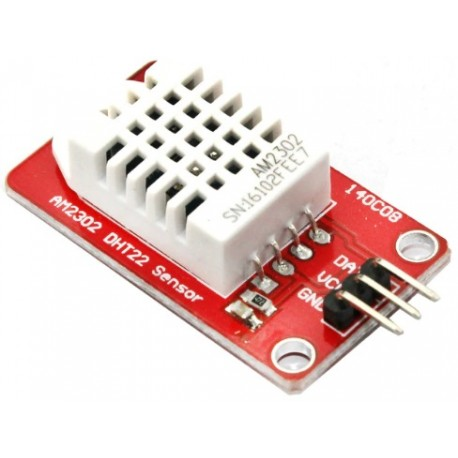
\includegraphics[width=5cm, height=5cm]{imagenes/dht22.jpg}
      \caption{Sensor DHT22}
      \subcaption*{Fuente: Datasheet fabricante}
      \label{imag:dht22}
    \end{figure}

Este sensor se encuentra presente en el submódulo 3 (ver figura \ref{imag:prueba_concepto}) de la prueba de concepto, ubicado en la parte superior de la vitrina,
logrando así obtener la mayor cantidad de valores de temperatura y humedad.
   
El DHT22 (AM2302) es un sensor digital de temperatura y humedad relativa de buen rendimiento y de bajo costo. Integra un sensor capacitivo de humedad y un termistor para medir el aire circundante, y muestra los datos mediante una señal digital en el pin de datos (no posee salida analógica).

Utiliza tecnología exclusiva de recolección de señales digitales y tecnología de detección de humedad, lo que garantiza su confiabilidad y estabilidad. Sus elementos de detección están conectados con una computadora de un solo chip de 8 bits.\\

\textbf{Especificaciones ténicas}

\begin{itemize}
    \item Modelo: AM2302
    \item Voltaje de alimentación: 3.3-6V DC
    \item Señal de salida: señal digital
    \item Rango: humedad de 0 - 100\%HR || temperatura de -40 - 125°C
\end{itemize}

\begin{figure}[H]
    \centering
    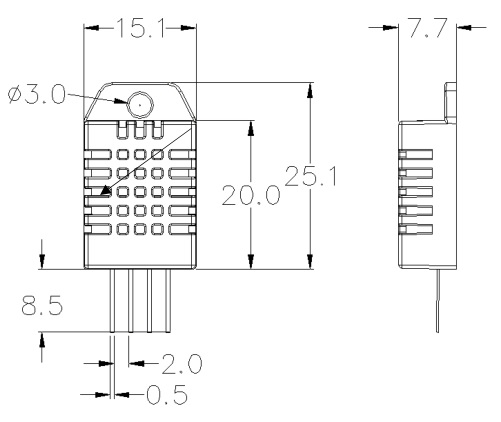
\includegraphics[width=8cm, height=6cm]{imagenes/dht22 dimensiones.jpg}
    \caption{Dimensiones sensor DHT22}
    \subcaption*{Fuente: Datasheet fabricante}
    \label{imag:dimensiones_dht22}
\end{figure}

Secuencia de números de pines: De izquierda a derecha 1,2,3,4 (tabla \ref{tab:pines_DHT})

\begin{table}[H]
    \centering
    \caption{Distribución pines DHT22}
    \label{tab:pines_DHT}
    \begin{tabular}{|l|l|}
    \hline
    Pin & Función            \\ \hline
    1   & VDD - Alimentación \\ \hline
    2   & DATA - Señal       \\ \hline
    3   & NULL               \\ \hline
    4   & GND                \\ \hline
    \end{tabular}
\end{table}

\subsection{Sensor de CO2 SGP30}

\begin{figure}[H]
      \centering
      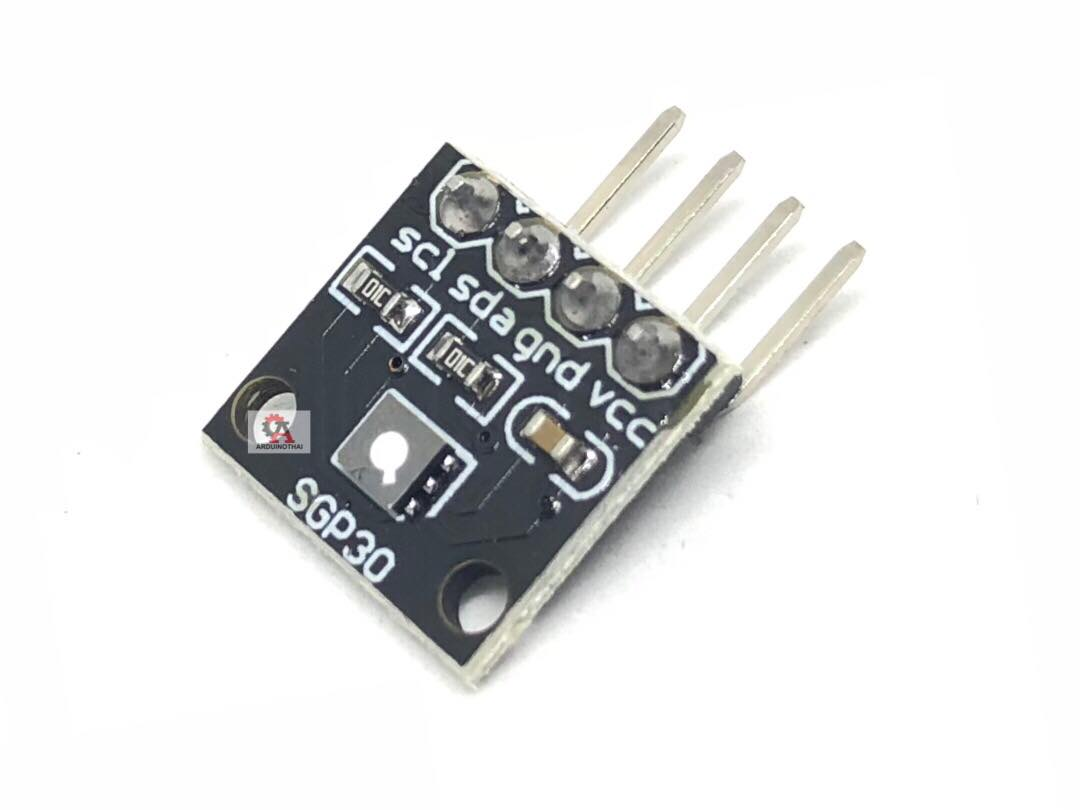
\includegraphics[width=6cm, height=4.5cm]{imagenes/sgp30.jpg}
      \caption{Sensor SGP30}
      \label{imag:sgp30}
\end{figure}

Este sensor, como parte de la prueba de concepto, se encuentra ubicado en el submódulo 1 (figura \ref{imag:prueba_concepto}), este debe estar ubicado en la parte superior de la vitrina, esto debido a que los gases tienden a subir \textbf{(referenciar)} y de esta manera se obtienen los valores de CO2 más exactos.

El SGP30 es un sensor de gas digital multipíxel diseñado para una fácil integración en purificadores de aire, ventilación controlada por demanda y aplicaciones IoT. La tecnología CMOSens® de Sensirion ofrece un sistema de sensor completo en un solo chip con una interfaz digital I 2C, una microplaca calefactora con control de temperatura y dos señales de calidad del aire interior preprocesadas. Como el primer sensor de gas de óxido de metal con múltiples elementos de detección en un chip, el SGP30 proporciona información más detallada sobre la calidad del aire.

El elemento sensor presenta una robustez inigualable contra los gases contaminantes presentes en las aplicaciones del mundo real, lo que permite una estabilidad única a largo plazo y una baja deriva. El paquete DFN muy pequeño de 2,45 x 2,45 x 0,9 mm3 permite aplicaciones en espacios limitados. El proceso de producción de vanguardia de Sensirion garantiza una alta reproducibilidad y confiabilidad. El empaque de cinta y carrete, junto con la idoneidad para los procesos de ensamblaje SMD estándar, hacen que el SGP30 esté predestinado para aplicaciones de alto volumen.

En la figura \ref{imag:diagrama_funcional} se observa el diagrama funcional del sensor SGP30.

\begin{figure}[H]
    \centering
    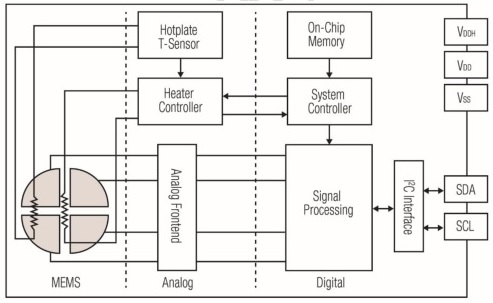
\includegraphics[width=9cm, height=5.7cm]{imagenes/diagrama_funcional_SGP30.jpg}
    \caption{Diagrama funcional SGP30}
    \subcaption*{Fuente: Datasheet fabricante}
    \label{imag:diagrama_funcional}
 \end{figure}

En la tabla \ref{tab:señales_calidad_aire} se muestran las especificaciones para los valores de calidad de aire en TVOC y CO2, a la salida del sensor SGP30.

\begin{table}[H]
    \centering
    \caption{Señales de calidad de aire}
    \subcaption*{Fuente: Datasheet fabricante}
    \label{tab:señales_calidad_aire}
    \begin{tabular}{|c|c|cc|}
    \hline
    \rowcolor[HTML]{9698ED} 
    \multicolumn{1}{|l|}{\cellcolor[HTML]{9698ED}Parámetro} & \multicolumn{1}{l|}{\cellcolor[HTML]{9698ED}Señal} & \multicolumn{2}{l|}{\cellcolor[HTML]{9698ED}Valores} \\ \hline
                                                            & Señal TVOC                                         & \multicolumn{2}{c|}{0 ppb a 60000 ppb}               \\ \cline{2-4} 
    \multirow{-2}{*}{Rango de salida}                       & Señal CO2eq                                        & \multicolumn{2}{c|}{400 ppm a 60000 ppm}             \\ \hline
                                                            &                                                    & \multicolumn{1}{c|}{0 ppb a 2008 ppb}       & 1 ppb  \\ \cline{3-4} 
                                                            &                                                    & \multicolumn{1}{c|}{2008 ppb – 11110 ppb}   & 6 ppb  \\ \cline{3-4} 
                                                            & \multirow{-3}{*}{Señal TVOC}                       & \multicolumn{1}{c|}{11110 ppb – 60000 ppb}  & 32 ppb \\ \cline{2-4} 
                                                            &                                                    & \multicolumn{1}{c|}{400 ppm – 1479 ppm}     & 1 ppm  \\ \cline{3-4} 
                                                            &                                                    & \multicolumn{1}{c|}{1479 ppm – 5144 ppm}    & 3 ppm  \\ \cline{3-4} 
                                                            &                                                    & \multicolumn{1}{c|}{5144 ppm – 17597 ppm}   & 9 ppm  \\ \cline{3-4} 
    \multirow{-7}{*}{Resolución}                            & \multirow{-4}{*}{Señal CO2eq}                      & \multicolumn{1}{c|}{17597 ppm – 60000 ppm}  & 31 ppm \\ \hline
                                                            & Señal TVOC                                         & \multicolumn{2}{c|}{1 Hz}                            \\ \cline{2-4} 
    \multirow{-2}{*}{Tasa de muestreo}                      & Señal CO2eq                                        & \multicolumn{2}{c|}{1 Hz}                            \\ \hline
    \end{tabular}
\end{table}

\textbf{Distribución pines de la interfaz}

La interfaz del sensor SGP30 del paquete DFN posee 6 pines como se muestra en la figura \ref{imag:interfaz_sgp30}. Para comprender esta figura se elabora la tabla \ref{tab:asignacion_pines} donde se le asigna a cada número la descripción correspondiente. A continuación la tabla \ref{tab:asignacion_pines}:

\begin{table}[H]
    \centering
    \caption{Asignación de pines}
    \subcaption*{Fuente: Datasheet fabricante}
    \label{tab:asignacion_pines}
    \begin{tabular}{|l|l|l|}
    \hline
    \rowcolor[HTML]{9698ED} 
    Pin & Nombre & Descripción                               \\ \hline
    1   & VDD    & Voltaje de alimentación                   \\ \hline
    2   & VSS    & Tierra                                    \\ \hline
    3   & SDA    & Data serial, bidireccional                \\ \hline
    4   & R      & Conectar a tierra (Sin función eléctrica) \\ \hline
    5   & VDDH   & Voltaje de alimentación (hotplate)        \\ \hline
    6   & SCL    & Reloj serial (bidireccional)              \\ \hline
    \end{tabular}
\end{table}

\begin{figure}[H]
    \centering
    \includegraphics[width=7cm, height=5.5cm]{imagenes/asignación_pines.jpg}
    \caption{Interfaz SGP30}
    \subcaption*{Fuente: Datasheet fabricante}
    \label{imag:interfaz_sgp30}
 \end{figure}

\subsection{Sensor de vibración TZT-LM393}

Para la instalación de este sensor se le anexó al submódulo 3 (figura \ref{imag:ubicacion_submodulo3}) un compartimiento donde estaría ubicado el mismo.

El módulo de la vibración basado en el sensor de vibración SW-420, modelo TZT y el comparador LM393 (figura \ref{imag:TZT}), sirve para detectar cualquier tipo de señal de vibración más allá del umbral de vibración.
Cuando no existen señales de vibración, este pequeño módulo se encarga de dar a conocer esto mediante un indicador LED de estado bajo y alto, según correspondiera; se caracteriza por tener una única señal de salida digital que
puede ser tratada mediante un dispositivo externo, como un microcontrolador, así se puede llevar a cabo una función específica.\\

\begin{figure}[H]
    \centering
    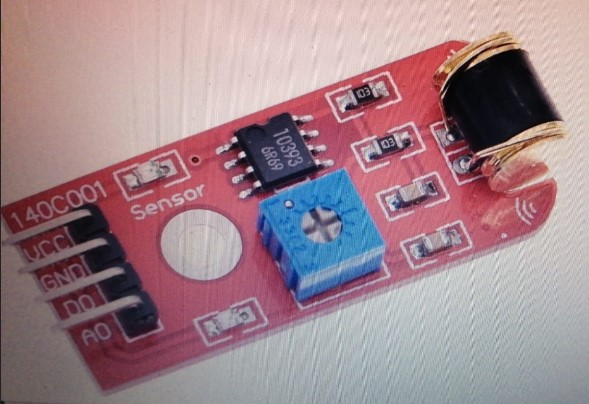
\includegraphics[width=6.5cm, height=5cm]{imagenes/sensor TZT.jpg}
    \caption{Sensor TZT-LM393}
    \label{imag:TZT}
\end{figure}

Este sensor posee características específicas que lo hacen idóneo para el análisis de los niveles de vibraciones presentes en la colección procedentes del exterior de la misma a causa, principalmente, del paso de los vehículos por la calle.\\

\textbf{Especificaciones}
\begin{itemize}
    \item El estado por defecto del interruptor es encendido
    \item Salida digital
    \item Voltaje de funcionamiento: 3.3V-5V
    \item Chip LM393
    \item Dimensiones: 3.2cm x 1.4cm
\end{itemize}

\subsection{Sensor de calidad de aire ZP07-MP503}

ZP07 air-quality module adopts flat surface semiconductor gas sensor. The module has good sensitivity to volatile organic gases such as formaldehyde, benzene, carbon
monoxide, ammonia, hydrogen, alcohol and smoke of cigarette, essence and etc. The module has been aging, debugged, adjusted and calibrated. So it has good consistency and high sensitivity.\\

\textbf{Características}
\begin{itemize}
    \item High sensitivity
    \item Low power consumption, long life
    \item Calibrated before shipment
    \item 10 seconds to 3 minutes with auto-preheating function
    \item Faulty auto-check, High cost-effective
\end{itemize}

\textbf{Aplicaciones}
\begin{itemize}
    \item Air cleaner, fresh-air system, intelligent integrated ceiling, air quality detector, ventilator, air-condition
\end{itemize}

\textbf{Distribución pines}

\begin{figure}[H]
    \centering
    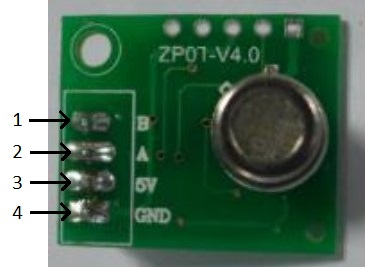
\includegraphics[width=6.5cm, height=5cm]{imagenes/sensor zp07.jpg}
    \caption{Sensor ZP07-MP503}
    \label{imag:ZP07}
\end{figure}

En la imágen anterior se aprecia la vista frontal del sensor de calidad de aire ZP07-MP503 con la numeración de los pines. Esta numeración se emplea en la tabla \ref{tab:pines_ZP07} para el análisis de la descripción de los mismos.

\begin{table}[H]
    \centering
    \caption{Distribución pines}
    \label{tab:pines_ZP07}
    \begin{tabular}{|l|l|l|}
    \hline
    \rowcolor[HTML]{9698ED} 
    Pin & Nombre & Función                          \\ \hline
    1   & GND    & Entrada de alimentación negativa \\ \hline
    2   & 5V     & Entrada de alimentación positiva \\ \hline
    3   & A      & Señal de salida A                \\ \hline
    4   & B      & Señal de salida B                \\ \hline
    \end{tabular}
\end{table}


\subsection{Sensor de luz BH1750}

El Módulo BH1750 es un sensor de iluminación digital para medición de flujo luminoso (iluminancia) de la empresa Rohm Semiconductor. Componente que posee dentro de su arquitectura interna, un conversor análogo digital (ADC) de 16 bits con una salida digital de formato I2C, que facilita la integración con microcontroladores o sistemas embebidos diversos. Este módulo entrega la intensidad luminosa directamente en unidades de Lux que es equivalente a Lumen/m2.\\

\begin{figure}[H]
    \centering
    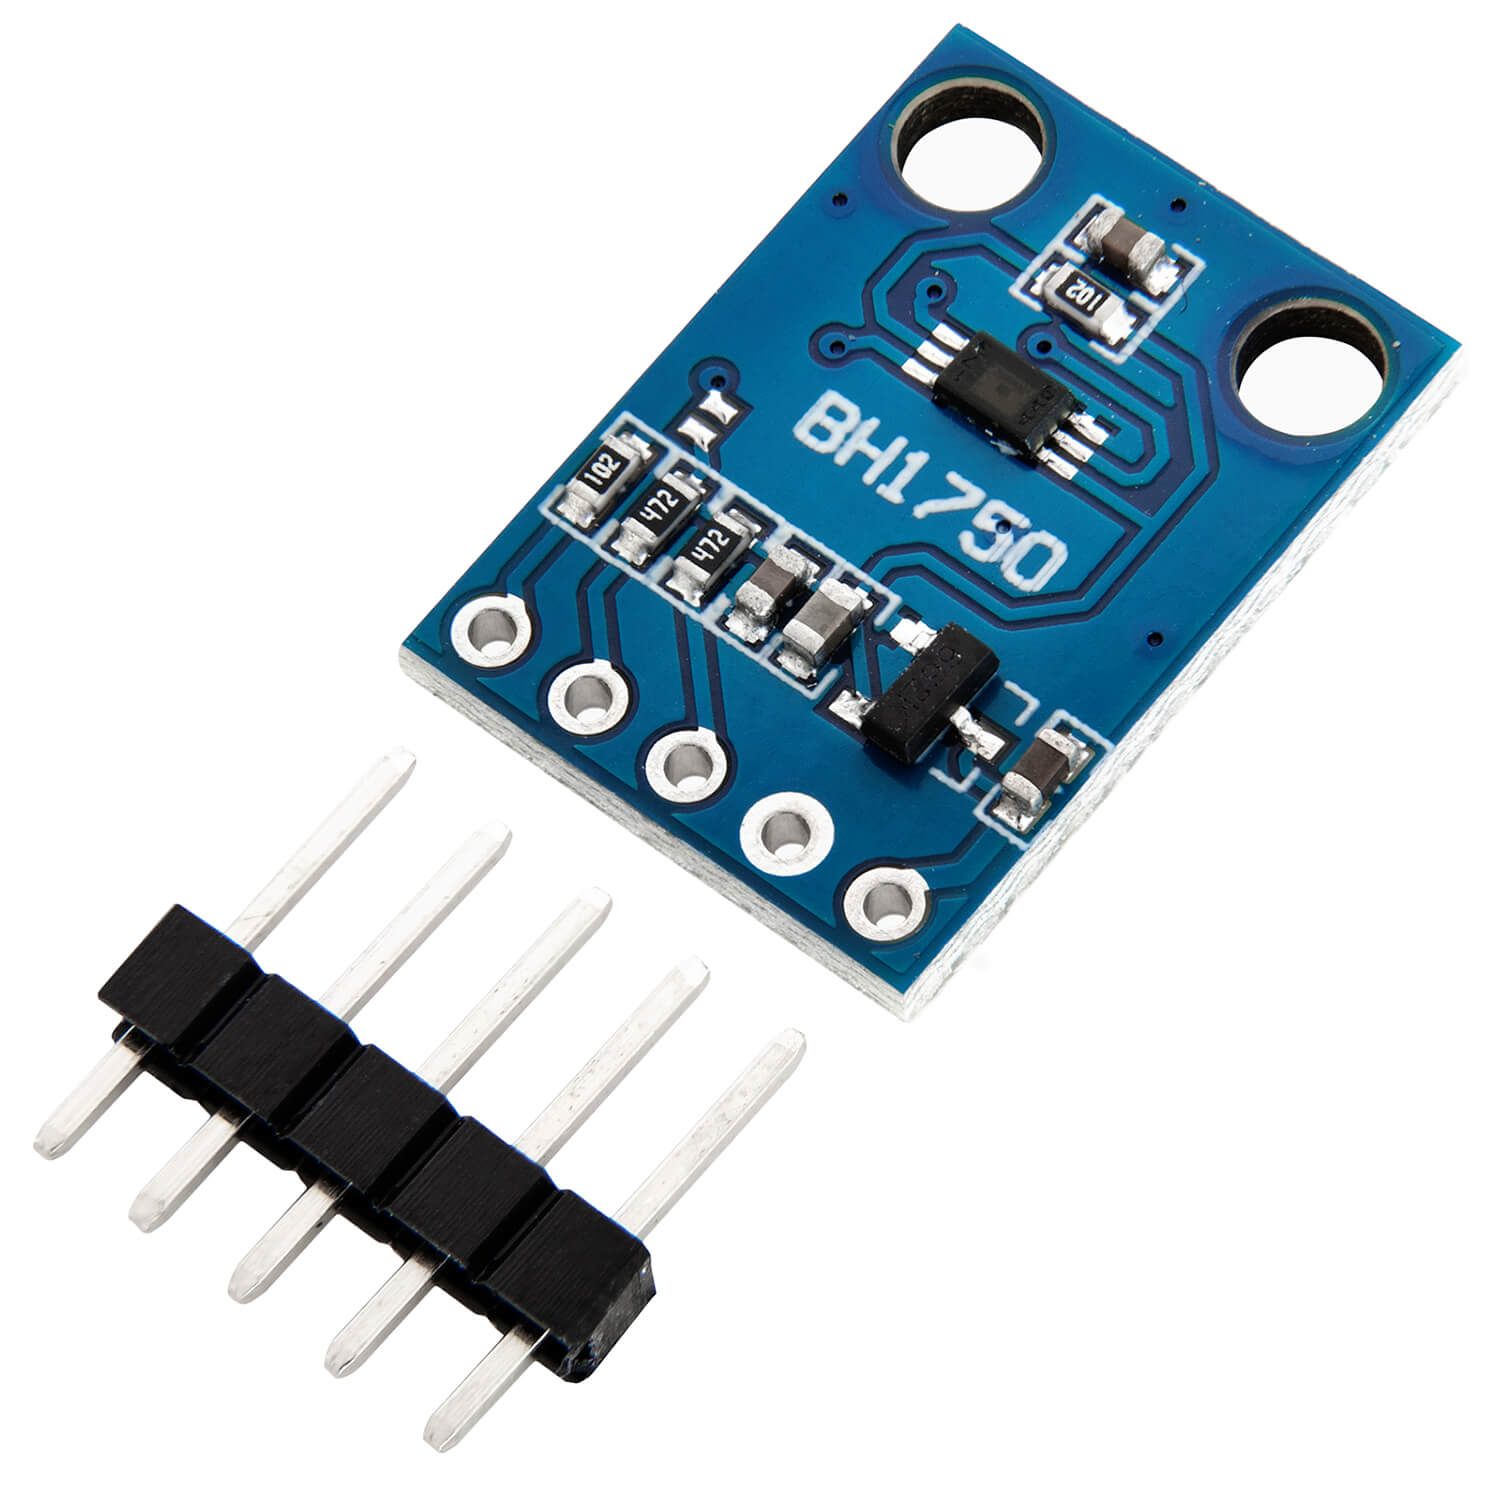
\includegraphics[width=5cm, height=4cm]{imagenes/Sensor BH1750.jpg}
    \caption{Sensor BH1750}
    \label{imag:BH1750}
 \end{figure}

\textbf{Otros datos}

\begin{itemize}
    \item Interfaz Digital: I2C
    \item Frecuencia máxima de transmisión: 400kHZ
    \item Temperatura de operación: Desde -40°C hasta 85°C
\end{itemize}

Para su correcto funcionamiento, este sensor debe ir acompañado de una serie de componentes electrónicos para su acondicionamiento.
En la figura \ref{imag:acondicionamiento_BH1750} se puede observar el acondicionamiento brindado por el fabricante.

\begin{figure}[H]
    \centering
    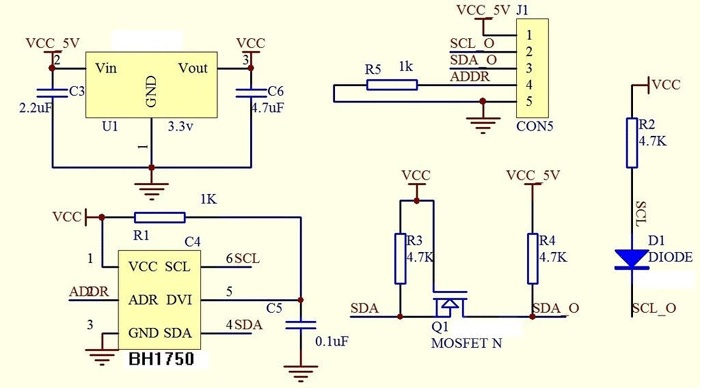
\includegraphics[width=11cm, height=7cm]{imagenes/acondicionamientos sensor BH1750.jpg}
    \caption{Acondicionamiento sensor BH1750}
    \subcaption*{Fuente: Datasheet fabricante}
    \label{imag:acondicionamiento_BH1750}
\end{figure}

\subsection{Módulo lector tarjetas SD}

...

\section{Arduino (IDE) y sensores}

Las conexiones entre el Nodo y los sensores se efectúa a través de conectores de tipo jack lo que brinda acceso a la posibilidad de agregar o extraer sensores sin complicaciones.

Esto hace que el trabajo con los sensores pase a un plano meramente programático, donde todo se desarrolla a través de código.

El IDE empleado para programar el hardware es el que brinda Arduino, ya que solo se necesita cargar el modelo de placa a programar.

Como se analizó antes, en el epígrafe \ref{subsec:sensores}, el valor de salida de los sensores es un voltaje que puede interpretarse como un valor de 0 a 1023 que se lee a través de los pines de entrada/salida analógicos.
Esta operación se realiza por medio de la función analogRead(), que admite como parámetro el pin analógico que se escoja para conectar con el sensor.

De los sensores que se emplean solo a tres de ellos se le efectuaron las calibraciones mediante el empleo de funciones \textit{map} almacenando los valores (mapeados) en arreglos (figura \ref{imag:mapeo_sensores}) ya que los demás poseen rangos de mínimos y máximos ya establecidos internamente.

\begin{figure}[H]
    \centering
    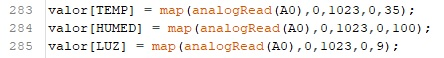
\includegraphics{imagenes/mapeado.jpg}
    \caption{Mapeo de los valores de los sensores}
    \label{imag:mapeo_sensores}
\end{figure}

En lo concerniente a Arduino se le llama mapeado al proceso de convertir los valores leídos de los pines en información útil. 

\section{Multiplexado}

Como parte de las deficiencias corregidas a través del diseño del nuevo prototipo de placa para los Nodos en las vitrinas (epígrafe \ref{subsec:nuevo_prototipo_nodo}) se incorpora un multiplexor en aras de ampliar la disponibilidad
de entradas analógicas para poder incorporar mayor cantidad de sensores con señales de salida de este tipo.

El multiplexor empleado (CD74HC4051) posee la característica de poder conectar varios sensores a un solo pin analógico.

El 74HC4051 es un multiplexor/demultiplexor de 8 bit...

...



\section{Alimentación}

Mediante la prueba de concepto, como ya se analizaba anteriormente, se determinó que el consumo de corriente era elevado, por ello, para el nuevo prototipo de Nodo para las vitrinas (subepígrafe \ref{subsec:nuevo_prototipo_nodo}) se 
incorpora un regulador de tipo LDO reduciendo grandemente el consumo de energía de este prototipo.\\

\textbf{Regulador LDO RT9013}

El RT9013 es un regulador LDO de 500 mA de alto rendimiento que ofrece PSRR extremadamente alto y caída ultrabaja. Ideal para aplicaciones inalámbricas y de RF portátiles con requisitos exigentes de rendimiento y espacio.

La corriente de reposo RT9013 es tan baja como 25uA, lo que prolonga aún más la vida útil de la batería. El RT9013 también funciona con condensadores cerámicos de baja ESR, lo que reduce la cantidad de espacio de placa necesario para las aplicaciones de energía, lo que es fundamental en los dispositivos inalámbricos de mano.

El RT9013 consume 0.7uA típicos en modo de apagado y tiene un tiempo de encendido rápido de menos de 40us. Las otras características incluyen voltaje de caída ultrabajo, alta precisión de salida, protección de limitación de corriente y alta relación de rechazo de ondulación. Disponible en el paquete SC-82, SOT-23-5, SC-70-5 y WDFN-6L 2x2.\\

\textbf{Características}

\begin{itemize}
    \item Amplios rangos de voltaje de operación: 2.2V a 5.5V
    \item Caída baja: 250mV a 500mA
    \item Ruido ultrabajo para aplicaciones de RF
    \item Respuesta ultrarrápida en transitorios de línea/carga
    \item Protección de limitación de corriente
    \item Protección de apagado térmico
    \item Tasa de rechazo de fuente de alimentación alta
    \item A la salida solo se requiere 1 uF de condensador para la estabilidad
    \item Entrada de apagado controlado por lógica TTL
\end{itemize}

\vspace{1cm}

\begin{figure}[H]
    \centering
    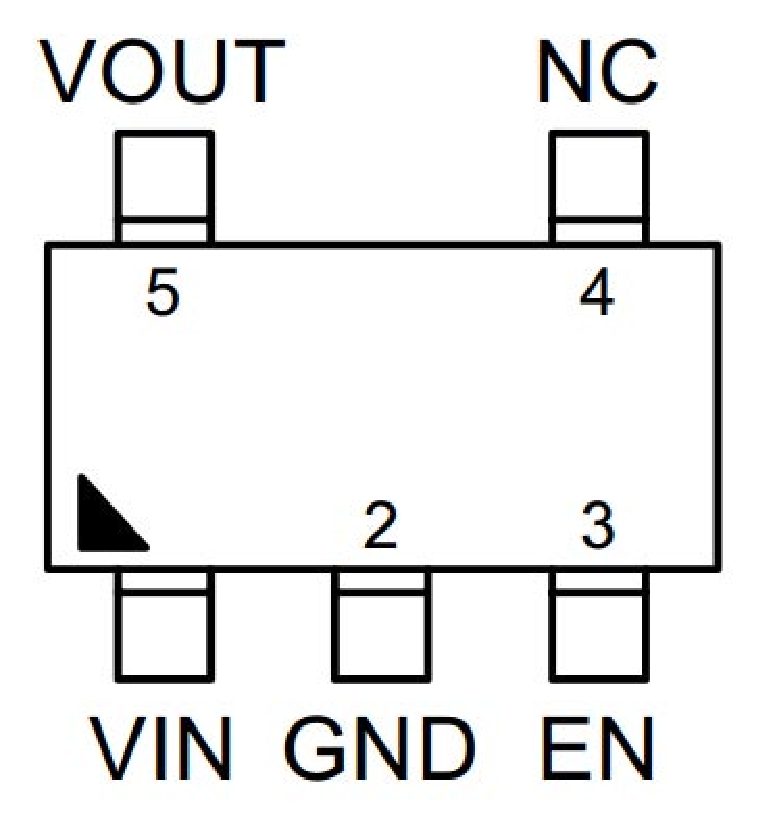
\includegraphics[width=4.5cm, height=5cm]{imagenes/esquematico RT9013.pdf}
    \caption{Configuración de pines}
    \subcaption*{Fuente: Datasheet fabricante}
    \label{imag:pines_RT9013}
\end{figure}

\begin{figure}[H]
    \centering
    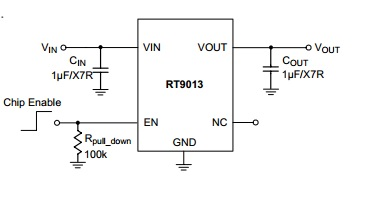
\includegraphics[width=11cm, height=6cm]{imagenes/acondicionamiento RT9013.jpg}
    \caption{Acondicionamiento}
    \subcaption*{Fuente: Datasheet fabricante}
    \label{imag:acondicionamiento_RT9013}
\end{figure}

\section{Evaluación económica}

Este proyecto se concibió para ajustarse siempre a la premisa de con el mínimo precio no sacrificar la calidad.

Esto del empleo de pequeños microcontroladores con programación libre se ha convertido en una alternativa para pequeñas empresas por su reducido costo y sus amplias aplicaciones, principalmente en aplicaciones de domótica, tal como el caso del sistema presentado.

Los precios en el mercado internacional de las tarjetas, kits, módulos y accesorios que conforman el sistema implementado, hacen que el desarrollo del mismo sea costeable y pueda ponerse en práctica en países en vías de desarrollo, como el nuestro.

En la siguiente tabla se relaciona lo que se considera como presupuesto mínimo del proyecto.

\begin{table}[H]
    \centering
    \caption{Relación de precios de los componentes del sistema}
    \label{tab:precios_componentes}
    \begin{tabular}{|l|l|r|}
    \hline
    \cellcolor[HTML]{9698ED}Elemento    & \cellcolor[HTML]{9698ED}Precio unitario  \\ \hline
    ESP-12F                             & ...                                      \\ \hline
    Sensor DHT22                        & \$3.82                                   \\ \hline
    Sensor SGP30                        & \$6.34                                   \\ \hline
    Sensor TZT-LM393                    & \$2.14                                   \\ \hline
    Sensor ZP07-MP503                   & \$2.22                                   \\ \hline
    Sensor BH1750                       & ...                                      \\ \hline
    Lector tarjeta SD                   & ...                                      \\ \hline
                                        & Total:                                   \\ \hline
    \end{tabular}
\end{table}

También se tuvo en cuenta el empleo de la mínima instrumentación, de tal forma que cuando se decida instalar el sistema, no se necesita adquirir nada más fuera de lo analizado para que se obtengan los datos esperados.
Los precios fueron tomados del mercado alternativo de Aliexpress\footnote{http://www.aliexpress.com}.\\

\addcontentsline{toc}{section}{Conclusiones capítulo 2}
        \textbf{\Large Conclusiones capítulo 2}\newline
